En juin 2019, une population de 200 marmottes a été introduite dans un massif montagneux où cette espèce était absente. Un zoologue en charge de ce projet souhaite modéliser l'évolution de cette population en fonction du temps.
	
	Il constate qu'entre juin 2019 et juin 2020, la population a augmenté de 20 individus.
	
	\subsection*{Partie A : Premier modèle}
	
	Le zoologue propose un premier modèle où la population augmente de 20 individus tous les ans.
	
	On note alors $u_{n}$ la population de marmottes que l'on peut estimer à l'aide de ce modèle en juin $2019+n$. On a donc $u_{0}=200$.
	
	\begin{enumerate}
		\item Quelle est la nature de la suite $\left(u_{n}\right)$ ? Préciser sa raison.
		
		\item À combien peut-on estimer le nombre de marmottes en juin 2025 ?
		
		\item En juin 2025, un nouveau décompte a permis de savoir que la population était de 355 individus. Ce premier modèle semble-t-il être adapté à la situation ?
	\end{enumerate}
	
	\subsection*{Partie B : Second modèle}
	
	\begin{enumerate}
		\item On rappelle que la population de marmottes était de 200 individus en juin 2019 et de 220 individus en juin 2020.
		
		De quel pourcentage la population a-t-elle augmenté entre ces deux dates ?
		
		\medskip
		
		Le zoologue propose un second modèle où la population augmente de ce même pourcentage tous les ans. Dans ce modèle, on représente la population de marmottes en juin $2019+n$ par $v_{n}$ tel que, pour tout entier naturel $n$,\quad $v_{n+1}=1,1\times v_{n}$.
		
		\item \begin{enumerate}
			\item Quelle est la nature de la suite $\left(v_{n}\right)$ ? Préciser sa raison et son premier terme.
			
			\item Exprimer $v_{n}$ en fonction de $n$.
		\end{enumerate}
		
		\item On utilise un tableur pour calculer les termes de la suite $\left(v_{n}\right)$.
		








\begin{center}
\tabcolwidth{1cm} 
\begin{tikzpicture}
\tableur[2]{A-L}
\celtxt*[align=center]{A}{1}{$ n $}
\celtxt*[align=center]{B}{1}{0}
\celtxt*[align=center]{C}{1}{1}
\celtxt*[align=center]{D}{1}{2}
\celtxt*[align=center]{E}{1}{3}
\celtxt*[align=center]{F}{1}{4}
\celtxt*[align=center]{G}{1}{5}
\celtxt*[align=center]{H}{1}{6}
\celtxt*[align=center]{I}{1}{7}
\celtxt*[align=center]{J}{1}{8}
\celtxt*[align=center]{K}{1}{9}
\celtxt*[align=center]{L}{1}{10}
\celtxt*[align=center]{A}{2}{$ v(n) $}
\celtxt*[align=center]{B}{2}{200}
\celtxt*[align=center]{C}{2}{220}
\celtxt*[align=center]{D}{2}{242}
\celtxt*[align=center]{E}{2}{266}
\celtxt*[align=center]{F}{2}{293}
\celtxt*[align=center]{G}{2}{322}
\celtxt*[align=center]{H}{2}{354}
\celtxt*[align=center]{I}{2}{390}
\celtxt*[align=center]{J}{2}{429}
\celtxt*[align=center]{K}{2}{472}
\celtxt*[align=center]{L}{2}{519}
\end{tikzpicture}
\end{center}	

		\begin{enumerate}
			\item Selon ce nouveau modèle, à combien peut-on estimer le nombre de marmottes en juin 2025 ?
			
			\item En utilisant la donnée fournie dans la question \textbf{3} de la partie \textbf{A}, ce nouveau modèle semble-t-il pertinent ?
			
			\item Au mois de juin de quelle année la population de marmottes de ce massif montagneux aura-t-elle dépassé 400 individus, selon ce modèle ?
		\end{enumerate}
	\end{enumerate}
